\chapter{Experimental Results}
\label{chap:result}

Defined at the end of the Chapter~\ref{chap:intro}, the four objectives of this thesis are to augment the COACH system with an emotional reasoning engine based on BayesACT so that the augmented system: (1) is designed in a portable and extensible way; (2) runs in real-time from the perspective of the user group; (3) provides at least a level of functional assistance of as high quality as the COACH; (4) is able to tune the prompts in some way according to the emotional state of a user. It has been showed in the Chapter~\ref{chap:design} and Chapter~\ref{chap:impl} that the system we developed is easy to be extended. Experiments conducted on the system show that an average latency of 46.79ms is caused by the Observer component of the system, 0.009ms by the Buffer, and 1.65s by the Updater. The overall average latency of the system is around 1.70s, which means that the system runs in real-time from the perspective of its user group. 

We demonstrate in this section by laboratory based tests that the system is also able to provide a level of functional assistance and to produce system prompts that have encoded to some extent the emotional state of the user. The tests were conducted on a PC running 64-bit Ubuntu 12.04 LTS, with AMD FX(tm)-6300 Six-Core Processor × 6 and NVIDIA GeForce GTX 650 Ti Graphics Card. A kinect camera was mounted above the sink area and was the only sensor of the system.

\section{Parameter Setup}
This paragraph explains how the values of threshold variables $distance$ and $difference$ used in the EPA-Calculator were assigned based on statistical results obtained from experiments as follows. Videos were recorded while a person washed her hands with different emotions in nine complete hand-washing trials. A total number of 13703 frames were extracted from the videos. For each frame, the distances between the person's two hands were computed. For each pair of neighbouring frames, the distances that the person's hands moved between the frames were calculated as well. Histograms of the two ``distances'' are shown in Figure~\ref{fig:histogram}. Note that in around 69\% of the frames, the distances between the user's hands falls into the range of $(8, 40]$. Note also that in around 70\% of frames, the distances the user's hands have moved from their positions in the last frames falls into the range of $(3.5, 17.5]$. Based on analysis of the the distributions of the two ``distances'', we assigned the values of variables used in the EPA-Calculator as following: $distance = \{-\infty, 0, 8, 40, 128, 160, +\infty\}$, $potency = \{-4.3, -4.3, 0, 1, 2, 4.3, 4.3\}$, $difference = \{-\infty, 0, 3.5, 17.5, 35, 70, +\infty\}$, and $activity = \{-4.3, -4.3, -2, -1, 0, 4.3, 4.3\}$. Table~\ref{table:param-setting} shows an overview of the values assigned to important variables in our tests of the system. 

%
% figure:Histograms 
\begin{figure}[htb]
\centering
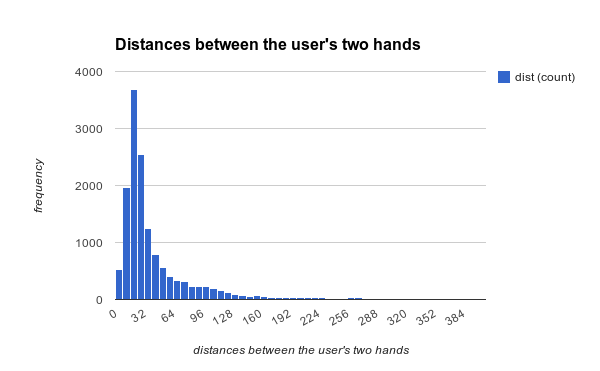
\includegraphics[width=0.9\linewidth]{fig/histogram1.png}
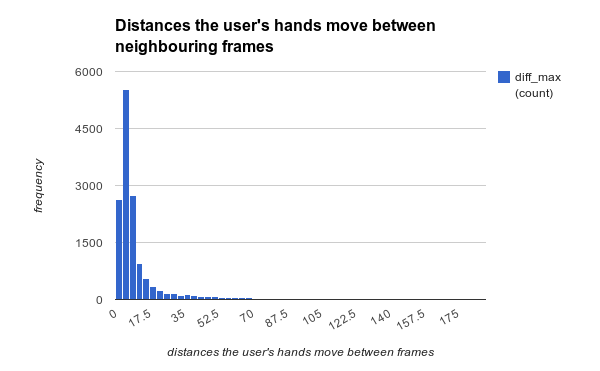
\includegraphics[width=0.9\linewidth]{fig/histogram2.png}
\caption{Histograms}
\label{fig:histogram}
\end{figure}


%
% table: Parameter values used in laboratory experiments
\begin{table}
\centering
\caption{Parameter values used in laboratory experiments}
\label{table:param-setting}
\begin{tabular}{| l | l | l |}
\hline
\textbf{Param.} & \textbf{Value} & \textbf{Defined in which component} \\ \hline
$n$ & $10$ & EPA-Calc \\ \hline
$distance$ & $\{-\infty, 0, 8, 40, 128, 160, +\infty\}$ & EPA-Calc \\ \hline
$potency$ & $\{-4.3, -4.3, 0, 1, 2, 4.3, 4.3\}$ & EPA-Calc \\ \hline 
$difference$ & $\{-\infty, 0, 3.5, 17.5, 35, 70, +\infty\}$ & EPA-Calc \\ \hline
$activity$ & $\{-4.3, -4.3, -2, -1, 0, 4.3, 4.3\}$ & EPA-Calc \\ \hline
$alpha$ & $0$ & Buffer \\ \hline
$timeout$ & $300$ & Buffer \\ \hline
$timeup$ & $1$ & Buffer \\ \hline
$\beta_{a}^{0}$ & $0.001$ & Updater \\ \hline
$\beta_{c}^{0}$ & $2.0$ & Updater \\ \hline
$\gamma$ & $(100000, 1.0, 0.5)$ & Updater \\ \hline
$N$ & $2000$ & Updater \\ \hline
$f\_a^{0}$ & $[1.5, 0.51, 0.45]$ & Updater \\ \hline
$f\_c^{0}$ & Different in each test &Updater \\ \hline
\end{tabular}
\end{table}

\section{Overview of Two Laboratory Tests}

%
% Table: results of test #1

\begin{longtable}{| V{0.8cm} | V{2.6cm} | V{1.6cm} | V{2.1cm} | V{1.55cm} | V{1.6cm} | V{3.2cm} |}
\caption{State changes in test \#1 of the system}
\label{table:result-1}

\\ \hline

Time &
User Behav. (screenshot) &
Behav. prop./epa &
Planstep Belief &
$f\_c$ &
Prompt: prop./epa &
Avatar (screenshot) \\ \hline
\endfirsthead

%column-1
t1 &
%column-2
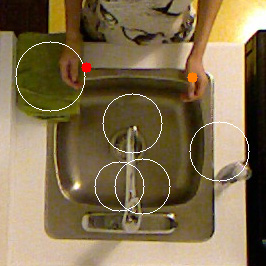
\includegraphics[width=\linewidth]{fig/system/_fast2-towel1_.jpg} &
%column-3
TOWEL
\linebreak\linebreak
$\begin{bmatrix}
0 \\
1.86 \\
-1.7
\end{bmatrix}$ &
%column-4
%\begin{minipage}[c]{\linewidth} \centering
[1.00, 0.00, 0.00, 0.00, 0.00, 0.00, 0.00, 0.00] most likely planstep=0
&
%\end{minipage} &
%column-5
$\begin{bmatrix}
1.7 \\
1.41 \\
-1.39
\end{bmatrix}$ &
%column-6
``turn on water''
\linebreak\linebreak
$\begin{bmatrix}
1.82 \\
0.22 \\
0.47
\end{bmatrix}$ &
%column-7
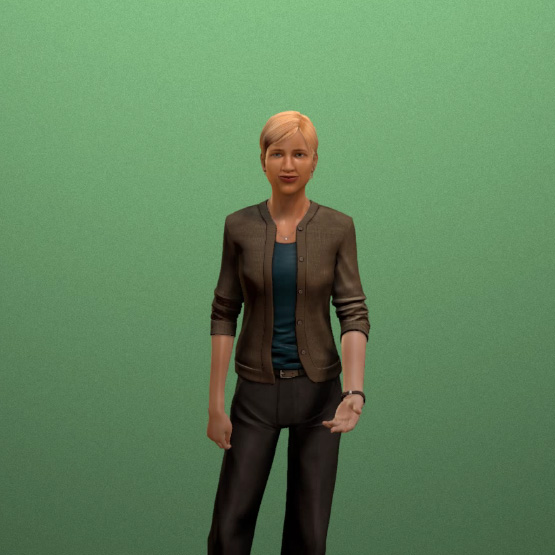
\includegraphics[width=2.6cm]{fig/prompt/_please-turn-on-the-water_.jpg}
\linebreak
\footnotesize
``Hello I am so glad to have you here. Please turn on the water.''
\\ \hline


%column-1
t2 &
%column-2
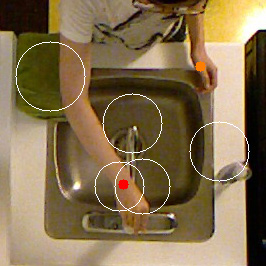
\includegraphics[width=\linewidth]{fig/system/_fast2-tap1_.jpg} &
%column-3
TAP
\linebreak\linebreak
$\begin{bmatrix}
0 \\
1.68 \\
-0.58
\end{bmatrix}$ &
%column-4
[0.26, 0.74, 0.00, 0.00, 0.00, 0.00, 0.00, 0.00] most likely planstep=1 &
%column-5
$\begin{bmatrix}
2.73 \\
1.14 \\
-1.03
\end{bmatrix}$ &
%column-6
N/A &
%column-7
No Prompt
\\ \hline


%column-1
t3 &
%column-2
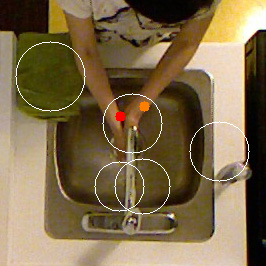
\includegraphics[width=\linewidth]{fig/system/_fast2-rinse1_.jpg} &
%column-3
RINSE
\linebreak\linebreak
$\begin{bmatrix}
0 \\
1.49 \\
-0.16
\end{bmatrix}$ &
%column-4
[0.27, 0.73, 0.00, 0.00, 0.00, 0.00, 0.00, 0.00] most likely planstep=1 &
%column-5
$\begin{bmatrix}
2.67 \\
1.21 \\
-0.72
\end{bmatrix}$ &
%column-6
``use some soap''
\linebreak\linebreak
$\begin{bmatrix}
1.51 \\
0.12 \\
0.52
\end{bmatrix}$ &
%column-7
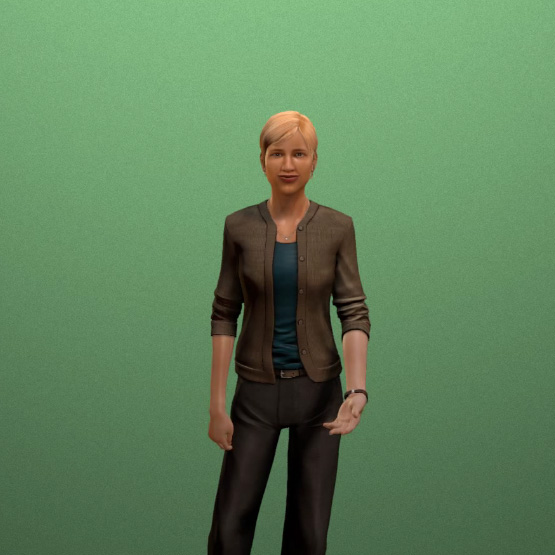
\includegraphics[width=2.6cm]{fig/prompt/_please-use-the-soap_.jpg}
\linebreak
\footnotesize
``You are washing your hands. Please use the soap.''
\\ \hline


%column-1
t4 &
%column-2
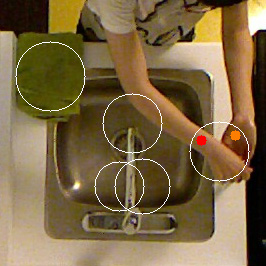
\includegraphics[width=\linewidth]{fig/system/_fast2-soap_.jpg} &
%column-3
SOAP
\linebreak\linebreak
$\begin{bmatrix}
0 \\
0.73 \\
-1.52
\end{bmatrix}$ &
%column-4
[0.00, 0.01, 0.35, 0.64, 0.00, 0.00, 0.00, 0.00] most likely planstep=3 &
%column-5
$\begin{bmatrix}
2.57 \\
0.69 \\
-0.66
\end{bmatrix}$ &
%column-6
N/A &
%column-7
No Prompt
\\ \hline


%column-1
t5 &
%column-2
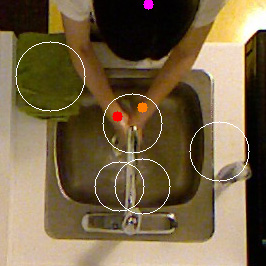
\includegraphics[width=\linewidth]{fig/system/_fast2-rinse_.jpg} &
%column-3
RINSE
\linebreak\linebreak
$\begin{bmatrix}
0 \\
0.23 \\
-1.87
\end{bmatrix}$ &
%column-4
[0.00, 0.00, 0.01, 0.02, 0.97, 0.00, 0.00, 0.00] most likely planstep=4 &
%column-5
$\begin{bmatrix}
2.92 \\
0.7 \\
-0.43
\end{bmatrix}$ &
%column-6
N/A &
%column-7
No Prompt
\\ \hline


%column-1
t6 &
%column-2
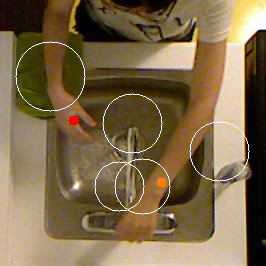
\includegraphics[width=\linewidth]{fig/system/_fast2-tap2_.jpg} &
%column-3
TAP
\linebreak\linebreak
$\begin{bmatrix}
0 \\
1.79 \\
-1.84
\end{bmatrix}$ &
%column-4
[0.00, 0.00, 0.00, 0.00, 0.18, 0.00, 0.82, 0.00] most likely planstep=6 &
%column-5
$\begin{bmatrix}
3.21 \\
0.98 \\
-0.47
\end{bmatrix}$ &
%column-6
N/A &
%column-7
No Prompt
\\ \hline


%column-1
t7 &
%column-2
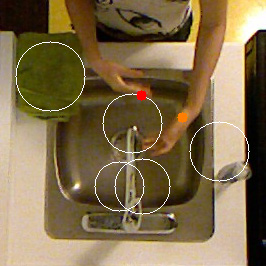
\includegraphics[width=\linewidth]{fig/system/_fast2-rinse3_.jpg} &
%column-3
RINSE
\linebreak\linebreak
$\begin{bmatrix}
0 \\
1.69 \\
-1.6
\end{bmatrix}$ &
%column-4
[0.00, 0.00, 0.00, 0.00, 0.21, 0.00, 0.79, 0.00] most likely planstep=6 &
%column-5
$\begin{bmatrix}
3.27 \\
1.07 \\
-0.58
\end{bmatrix}$ &
%column-6
``use towel''
\linebreak\linebreak
$\begin{bmatrix}
1.77 \\
0.16 \\
1
\end{bmatrix}$ &
%column-7
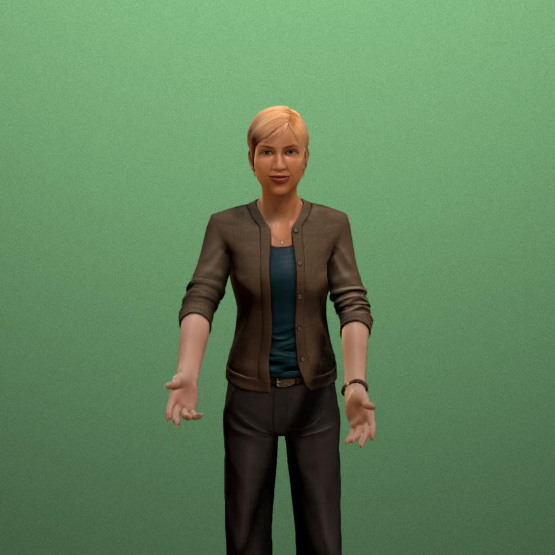
\includegraphics[width=2.6cm]{fig/prompt/_can-i-get-your-hands-dried-up_.jpg}
\linebreak
\footnotesize
``Can I get your hands dried up?''
\\ \hline


%column-1
t8 &
%column-2
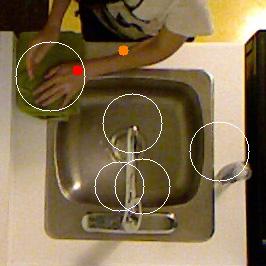
\includegraphics[width=\linewidth]{fig/system/_fast2-towel2_.jpg} &
%column-3
TOWEL
\linebreak\linebreak
$\begin{bmatrix}
0 \\
1.08 \\
-1.16
\end{bmatrix}$ &
%column-4
[0.00, 0.00, 0.00, 0.00, 0.00, 0.14, 0.00, 0.86] most likely planstep=7 &
%column-5
$\begin{bmatrix}
3.31 \\
1.04 \\
-0.57
\end{bmatrix}$ &
%column-6
``all done''
\linebreak\linebreak
$\begin{bmatrix}
1.55 \\
0.38 \\
0.87
\end{bmatrix}$ &
%column-7
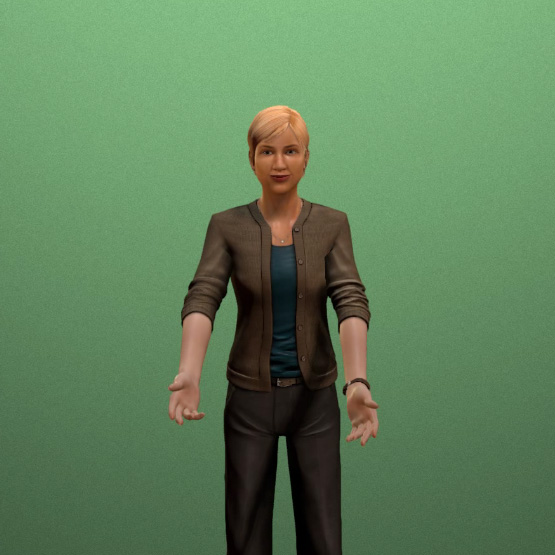
\includegraphics[width=2.6cm]{fig/prompt/_can-you-come-back-soon_.jpg}
\linebreak
\footnotesize
``Can you come back soon?''
\\ \hline

\end{longtable}



%
% Table: results of test #2

\begin{longtable}{| V{0.8cm} | V{2.6cm} | V{1.6cm} | V{2.1cm} | V{1.55cm} | V{1.6cm} | V{3.2cm} |}
\caption{State changes in test \#2 of the system}
\label{table:result-2}
\\ \hline


Time &
User Behav. (screenshot) &
Behav. prop./epa &
Planstep Belief &
$f\_c$ &
Prompt: prop./epa &
Avatar (screenshot) \\ \hline
\endfirsthead

%column-1
t1 &
%column-2
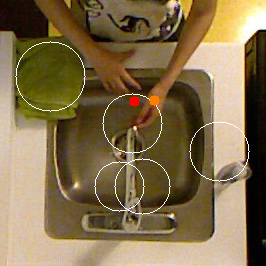
\includegraphics[width=\linewidth]{fig/system/_slow2-rinse1_.jpg} &
%column-3
RINSE
\linebreak\linebreak
$\begin{bmatrix}
0 \\
0.29 \\
-1.86
\end{bmatrix}$ &
%column-4
[1.00, 0.00, 0.00, 0.00, 0.00, 0.00, 0.00, 0.00] most likely planstep=0 &
%column-5
$\begin{bmatrix}
-0.87 \\
-0.28 \\
-2.11
\end{bmatrix}$ &
%column-6
``turn on water''
\linebreak\linebreak
$\begin{bmatrix}
0.87 \\
0.85 \\
0.27
\end{bmatrix}$ &
%column-7
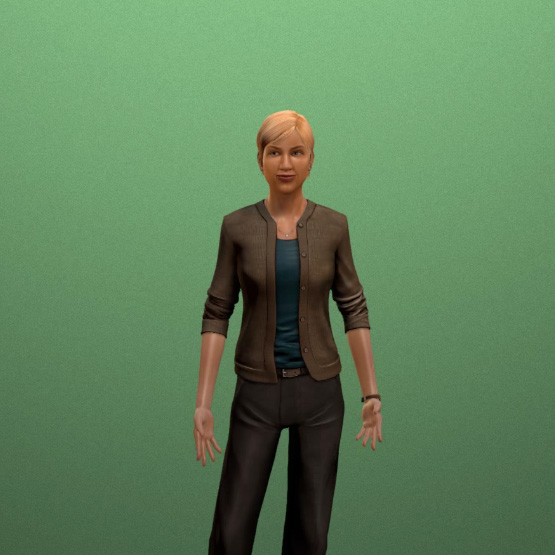
\includegraphics[width=2.6cm]{fig/prompt/_i-want-you-to-turn-the-water-on_.jpg}
\linebreak
\footnotesize
``I want you to turn the water on.''
\\ \hline


%column-1
t2 &
%column-2
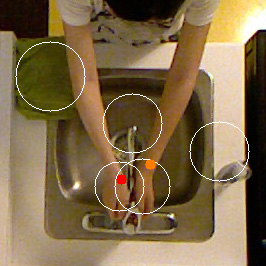
\includegraphics[width=\linewidth]{fig/system/_slow2-tap1_.jpg} &
%column-3
TAP
\linebreak\linebreak
$\begin{bmatrix}
0 \\
1.49 \\
-1.63
\end{bmatrix}$ &
%column-4
[0.46, 0.54, 0.00, 0.00, 0.00, 0.00, 0.00, 0.00] most likely planstep = 1 &
%column-5
$\begin{bmatrix}
-0.02 \\
-0.47 \\
-1.84
\end{bmatrix}$ &
%column-6
N/A &
%column-7
No Prompt
\\ \hline


%column-1
t3 &
%column-2
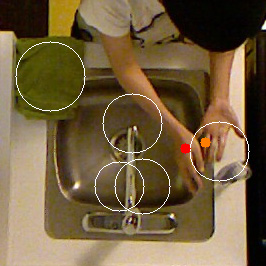
\includegraphics[width=\linewidth]{fig/system/_slow2-soap_.jpg} &
%column-3
SOAP
\linebreak\linebreak
$\begin{bmatrix}
0 \\
1.25 \\
-1.74
\end{bmatrix}$ &
%column-4
[0.02, 0.02, 0.24, 0.73, 0.00, 0.00, 0.00, 0.00] most likely planstep = 3 &
%column-5
$\begin{bmatrix}
1.2 \\
-0.37 \\
-1.46
\end{bmatrix}$ &
%column-6
N/A &
%column-7
No Prompt
\\ \hline


%column-1
t4 &
%column-2
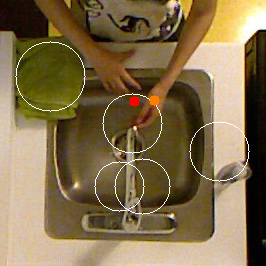
\includegraphics[width=\linewidth]{fig/system/_slow2-rinse1_.jpg} &
%column-3
RINSE
\linebreak\linebreak
$\begin{bmatrix}
0 \\
0.05 \\
-1.85
\end{bmatrix}$ &
%column-4
[0.00, 0.00, 0.00, 0.01, 0.98, 0.00, 0.00, 0.00] most likely planstep = 4 &
%column-5
$\begin{bmatrix}
1.66 \\
-0.46 \\
-1.32
\end{bmatrix}$ &
%column-6
N/A &
%column-7
No Prompt
\\ \hline


%column-1
t5 &
%column-2
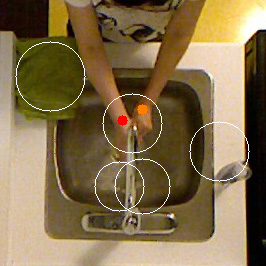
\includegraphics[width=\linewidth]{fig/system/_slow2-rinse2_.jpg} &
%column-3
RINSE
\linebreak\linebreak
$\begin{bmatrix}
0 \\
0.32 \\
-1.95
\end{bmatrix}$ &
%column-4
[0.00, 0.00, 0.00, 0.01, 0.98, 0.00, 0.00, 0.00] most likely planstep = 4 &
%column-5
$\begin{bmatrix}
1.61 \\
-0.45 \\
-1.33
\end{bmatrix}$ &
%column-6
``turn off water''
\linebreak\linebreak
$\begin{bmatrix}
1.88 \\
0.75 \\
0.38
\end{bmatrix}$ &
%column-7
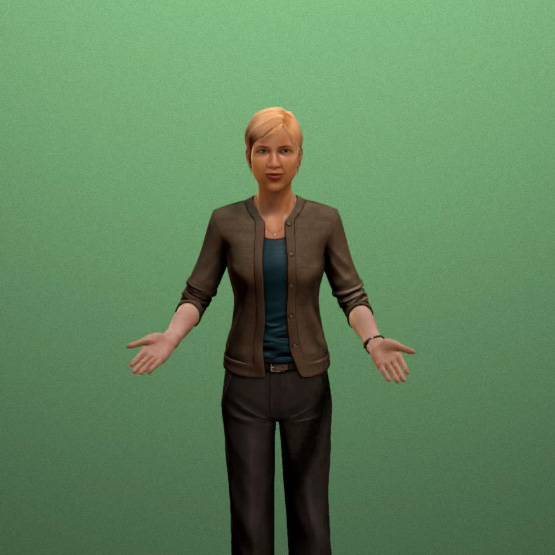
\includegraphics[width=2.6cm]{fig/prompt/_try-turning-off-the-water_.jpg}
\linebreak
\footnotesize
``Try turning off the water.''
\\ \hline



%column-1
t6 &
%column-2
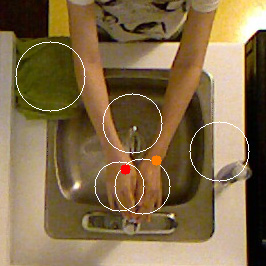
\includegraphics[width=\linewidth]{fig/system/_slow2-tap2_.jpg} &
%column-3
TAP
\linebreak\linebreak
$\begin{bmatrix}
0 \\
1.22 \\
-1.75
\end{bmatrix}$ &
%column-4
[0.00, 0.00, 0.00, 0.01, 0.18, 0.00, 0.81, 0.00] most likely planstep = 6 &
%column-5
$\begin{bmatrix}
1.84 \\
-0.48 \\
-1.25
\end{bmatrix}$ &
%column-6
N/A &
%column-7
No Prompt
\\ \hline


%column-1
t7 &
%column-2
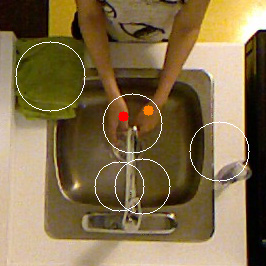
\includegraphics[width=\linewidth]{fig/system/_slow2-rinse3_.jpg} &
%column-3
RINSE
\linebreak\linebreak
$\begin{bmatrix}
0 \\
1.03 \\
-1.73
\end{bmatrix}$ &
%column-4
[0.00, 0.00, 0.00, 0.01, 0.29, 0.00, 0.70, 0.00] most likely planstep = 6 &
%column-5
$\begin{bmatrix}
1.77 \\
-0.46 \\
-1.25
\end{bmatrix}$ &
%column-6
``use towel''
\linebreak\linebreak
$\begin{bmatrix}
1.68 \\
0.82 \\
-0.16
\end{bmatrix}$ &
%column-7
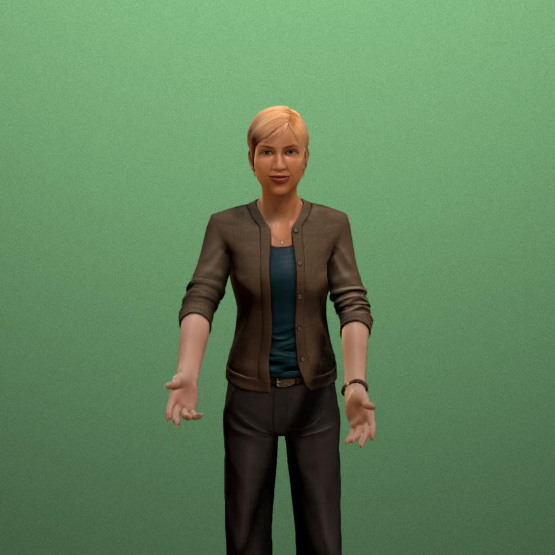
\includegraphics[width=2.6cm]{fig/prompt/_can-i-get-your-hands-dried-up_.jpg}
\linebreak
\footnotesize
``Can I get your hands dried up?''
\\ \hline


%column-1
t8 &
%column-2
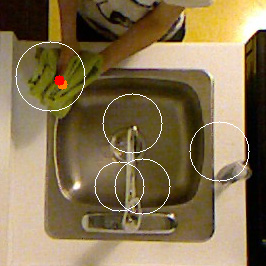
\includegraphics[width=\linewidth]{fig/system/_slow2-towel_.jpg} &
%column-3
TOWEL
\linebreak\linebreak
$\begin{bmatrix}
0 \\
0.48 \\
-1.42
\end{bmatrix}$ &
%column-4
[0.00, 0.00, 0.00, 0.00, 0.00, 0.09, 0.00, 0.91] most likely planstep = 7 &
%column-5
$\begin{bmatrix}
1.83 \\
-0.45 \\
-1.24
\end{bmatrix}$ &
%column-6
``all done''
\linebreak\linebreak
$\begin{bmatrix}
1.5 \\
0.6 \\
-0.03
\end{bmatrix}$ &
%column-7
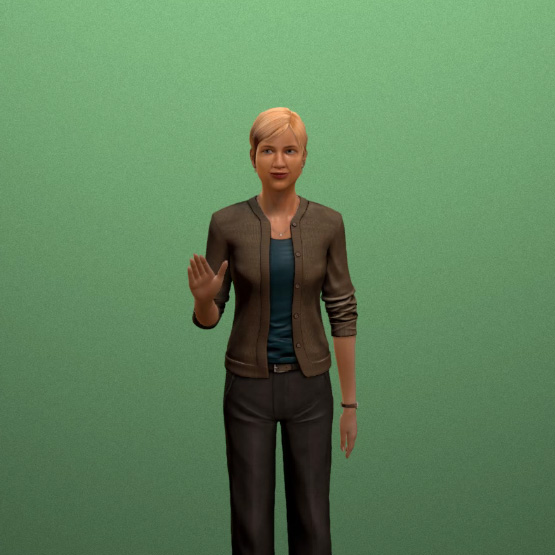
\includegraphics[width=2.6cm]{fig/prompt/_hope-to-see-you-soon_.jpg}
\linebreak
\footnotesize
``Good bye. Hope to see you soon.''
\\ \hline

\end{longtable}


Tables~\ref{table:result-1} and ~\ref{table:result-2} show the state changes of the system in two laboratory tests. In both of these tests, an actor was washing her hands while the system observes and assists her in real time. The difference between the two was that the actor acted more powerfully (with her hands more ``open'') and more actively (with her hands moving more quickly) in the first test than in the second one. $f\_c^0$ was set to $[1.61, 0.84, -0.87]$ (i.e. close to the EPA value of an identity of ``elder'') in test \#1, and was set to $[-0.64, -0.43, -1.81]$ (i.e. close to the EPA value of an identity of a ``lonesome elder'') in test \#2. As for the data in the tables, except for columns ``times'' and ``user behaviour (screenshot)'', all data in the table were computed by the system. The column "Planstep Belief" uses the definition of plansteps shown in Table~\ref{table:heuristic-policy}. The video prompts displayed by the system during the tests are described in the table by screenshots and the avatar's lines. As shown in the tables, the Planstep and Emotion Updater (i.e. the BayesAct reasoning engine) updated its states for a total of 8 times in both test \#1 and test \#2. We explain using the tables in the remaining of this section that the system is able to work both functionally and emotionally by looking at the experimental results of the two tests more closely.

\section{Functionality Performance of the System}

To make sure that the hand-washing system works well functionally, the following three aspects should be assured: (1) the system recognizes user-behaviours correctly; (2) it updates its beliefs of plansteps appropriately; (3) it could give out helpful prompts based on the belief states (i.e. the prompts should be propositionally useful). Recall that the first aspect depends on the performance of the Observer, and the last two aspects depends on that of the Planstep Updater. The column ``user behaviour screenshot'' in Tables ~\ref{table:result-1} and ~\ref{table:result-2} illustrates some screenshots of the system recognizing the actor's hands. As shown in the figures, the Observer extended from the original tracker is able to extract the positions of the user's hands when the user is turning on/off the tap, using soap, rinsing hands, and using towel. At each timestep, the Planstep Updater updates its planstep beliefs and computes a most likely planstep. Depending on the ``most-likely planstep'' computed, the Planstep Updater then decides (using the heuristic policy) on the propositional content of the system prompt at that time. For a certain most-likely planstep, the propositional content of the system prompt is deterministic. The policy based on which the propositional content of a system prompt is determined is shown in Table~\ref{table:heuristic-policy}.

Table~\ref{table:result-1} shows how the system's planstep beliefs and prompts were changed according to the user's behaviours in test \#1. At time t1, the actor was about to start washing her hands, with her right hand accidently being in the region of the towel. Observing this, the system thought the actor was using the towel, and concluded that the actor needed some instructions. The system suggested the user to turn on the water at t1. At time t2, the actor turned on the water. The system updated its planstep beliefs accordingly and got a most-likely planstep of 1. The system did not perform any prompts at t2, since it believed that the user had a high level of awareness (because she ``followed'' the system instructions) and was able to continue the handwashing task properly by herself. At time t3, the actor tried to rinse her hands. The system detected this behaviour of the actor and suggested her to put on some soap first. Then, at times t4, t5, and t6, the system updated its planstep beliefs and did not perform any prompts when the actor put on some soap (at t4), rinsed her hands (at t5) and turned off the water (at t6). At t7, the actor was detected as rinsing her hands again, while in fact she was just moving her hands from the tap area to the towel area. Believing that the actor had a low awareness level and was in need of some assistance, the system suggested the user to proceed with using the towel. At time t8, the actor finally completed the handwashing task, and the system prompted an ``all done'' message to indicate the accomplishment.

Table~\ref{table:result-1} shows how the system's planstep beliefs and prompts were changed according to the user's behaviours in test \#2. At time t1, the actor was detected as rinsing her hands while she was moving her hands towards the tap to turn on the water. The actor got an instruction suggesting her to turn on the water from the system. At time t2, the actor ``followed'' the system's instruction and turned on the water. The system updated its planstep beliefs accordingly and got a most-likely planstep of 1. The system did not perform any prompts at t2, since it believed that the user had a high level of awareness and was able to continue the handwashing task properly by herself. At times t3 and t4, the actor put on some soap and started rinsing her hands. The system updated its planstep beliefs and did not perform any prompts. At t5, the actor continued rinsing her hands. Believing that the actor having been performing the same behaviour for too long a time, which implied a low awareness level of the actor, the system suggested the user to proceed with turning off the water. The actor followed the system's instruction and turned off the water at time t6. At time t7, the actor performed the behaviour of rinsing her hands again. Believing that the actor had a low awareness level and was in need of some assistance, the system instructed suggested the user to use the towel. At time t8, the actor finally completed the handwashing task, and the system prompted an ``all done'' message to indicate the accomplishment. 

As shown in Tables~\ref{table:result-1} and ~\ref{table:result-2}, though the system sometimes might false positively recognize an user behaviour (e.g. thinking the actor was using the towel at t1 in test \#1), in general, it is able to produce propositionally useful system prompts in the two tests. The defection of falsely recognizing noise behaviours can be ameliorated by increasing the value of the parameter $timeup$, which is defined in the Buffer and is designed to handle (to some extent) behaviour noises. Readers can find state change details in a total of 17 tests, including the two shown in Tables~\ref{table:result-1} and ~\ref{table:result-2} and 15 other runs, conducted on the system in the appendix of this thesis.


\section{Emotionality Performance of the System}

To demonstrate that the system is able to work emotionally, this subsection compares the average of EPA values computed for user behaviours, for $f\_c$'s, and for system prompts in tests \#1 and \#2. Table~\ref{table:compare-epa-the-two} shows a simple comparison of the EPA values in the two aforementioned tests. 

%
% table: Comparison of EPA values in the two tests
\begin{table}
\centering
\caption{Comparison of EPA values in the two tests}
\label{table:compare-epa-the-two}
\begin{tabular}{|  p{0.7cm} | p{2.5cm} |  p{3.0cm} |  p{3.0cm} |  p{3.0cm} | p{2.6cm} |}
\hline
\footnotesize
Test & mean of User Behaviour & init of f\_c & final of f\_c & mean of f\_c & mean of system prompt \\ \hline
t1 & $[0,1.32,-1.3]$ & $[1.61,0.84,-0.87]$ & $[3.31,1.04,-0.57]$ & $[2.8,1.03,-0.73]$ & $[1.62,0.32,0.75]$ \\ \hline
t2 & $[0,0.77,-1.74]$ & $[-0.64,-0.43,-1.81]$ & $[1.83,-0.45,-1.24]$ & $[1.13,-0.43,-1.47]$ & $[1.53,0.66,0.08]$ \\ \hline
\end{tabular}
\end{table}

